\chapter{Introduction}
	\section{Active electronically scanned array}
		Radars of today often utilize a phased array function which permits steering of the antenna lobe by use of constructive and destructive interference. This removes the need for mechanical constructions that rotates the radar. By not having any movable parts, the reliability and performance vastly outperforms the properties of rotating radars. For example, because the angular speed of the electronically steered antenna array, the antenna lobe can simultaneously keep track of several targets while also scanning the skies for new ones. This type of radar is an electronically steered antenna, or ESA.\autocite{web:navair02}

		An ESA-antenna consists of many small antenna elements, or transmit/receive-modules. The signal's phase and amplitude are controlled individually for each TRM while other signal processing is common for groups of modules. It is therefore to one's advantage to create small antenna elements as well as small circuits controlling them. This can be done with monolithic microwave integrated circuits (or MMICs). MMICs are small, efficient and reliable, making them well-suited for radar applications.\autocite{stimson98}

		Older ESA's were usually passive (PESA); all TRMs operating at the same frequency and powered by a common source. If small groups of antenna elements are powered individually the array is active, an AESA. This gives the flexibility of being able to transmit over different frequencies at the same time and thus, amongst other things, decrease the likelihood of discovery.\autocites{oliner72}

		Common modern radars transmit at frequencies from \unit[1]{GHz} up to tens of GHz. Early digital sampling of the analogue signal enables more processing to be done in software, extending the radar's applications and utility. To perform analogue-to-digital conversion with today's technology, the frequency must be in the order of \unit[100]{MHz}. This is at least one order of magnitude less than the transmit frequencies.

		Figure \ref{fig:intro_fig} presents a usual setup of an AESA-system. The signal is received in a large number of TRM-modules where amplification and phase steering are performed. In the next step, the signal is prepared for AD-conversion by down-converting the frequency. In the third step, the signal is digitized and processed in software.

		In this thesis work, the first in a chain of necessary down-converters is designed on a GaAs MMIC. The chip is called multi-functional because it contains additional components such as amplifiers and variable attenuators. Due to the tailored performance with strict specifications and the inclusion of many components, the chip cannot be bought off the shelf. The main reason for implementing on an MMIC is the need for miniaturisation as it is important to start processing the signal as close to the antenna as possible.

		\begin{figure}[hpt!]
			\centering
			\subfloat[][]{
				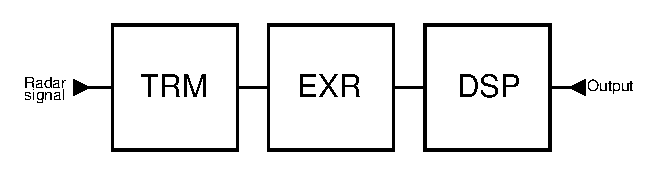
\includegraphics[width=0.7\textwidth]{fig/introduction/receiver}
				\label{fig:introreceiver}
			}\\
			\subfloat[][]{
				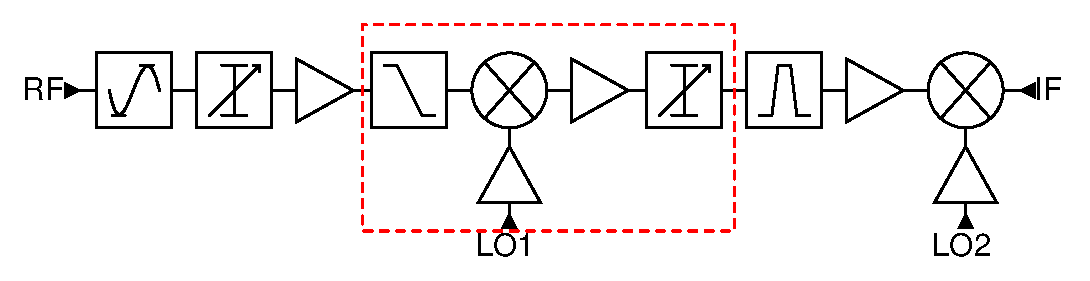
\includegraphics[width=1.0\textwidth]{fig/introduction/exr}
				\label{fig:introexr}
			}
			\caption[AESA receiver system.]{Schematic view of the AESA receiver system. \subref{fig:introreceiver} The signal is picked up by the antenna in the transmitter receiver module (TRM), processed in the exciter receiver subsystem (EXR) and finally converted to a digital signal in the DSP-unit, where digital beam forming is performed. \subref{fig:introexr} A detailed view of the EXR-unit. It contains a series of down-converters and filters. The down-converters are necessary to provide the analogue-to-digital converter with the correct frequency. This master's thesis covers the implementation of the first down-converter and a dynamic gain on an MMIC (components enclosed by a red dashed line). The chip is designed for the S band and contains image reject features. RF, LO and IF are explained in \nameref{ch:introduction_mixer} \ref{ch:introduction_mixer}.}\label{fig:intro_fig}
		\end{figure}

		%To perform analogue-to-digital conversion with today's technology, the frequency should preferably be at least one order of magnitude smaller than the carrier frequency (radio frequency or RF) of a radar which transmits/receives at \unit[3]{GHz}. In this thesis work the first in a chain of necessary down-converters will be designed on a GaAs MMIC.

	\section{Design specifics}
		As previously mentioned there is a need for a custom, very small, mixing circuit. Implementation as an integrated circuit is clearly beneficial because of the small size. In \autoref{app:specs} the full specification of the MMIC is listed. Most important are the demands on linearity, noise and gain. The gain is set to \unit[$\sim$10]{dB} with a \unit[$\pm$5]{dB} dynamic gain range. This means that the gain is variable and that the chip needs amplifiers and some means of controlling the gain. The linearity, measured using the input third-order intercept point, should be at least \unit[15]{dBm} at nominal gain. The noise figure should for nominal gain be less than \unit[15]{dB}. These quantities are explained later on in this chapter.


	\section{GaAs monolithic microwave integrated \\circuit}
		\subsection{Properties}

		MMICs offers miniaturization of electric circuits and can be constructed with different materials having different properties. Gallium arsenide (GaAs) has been used as a semiconductor material since the 70's. When it was introduced, it was a minor revolution; the high electron mobility permitted frequencies in excess of \unit[200]{GHz} and greater breakdown voltages increased the power levels. GaAs circuits are less sensitive to heat compared to ordinary silicon semiconductor materials and offers good noise-performance.\autocite{robertson95} %page 10

		\subsection{HEMT-technology}
			The active components of MMICs are usually FETs and different processes offer different kinds of FETs.	The High Electron Mobility Transistor-, or HEMT-technology uses the quantum well created in the conduction band in the interaction between two semiconductors. The electrons in the well form a two-dimensional electron gas that can be used to form the channel region of the FET.\autocite{mimura80} The two semiconductor-materials usually must have the same lattice constants.

			Pseudomorphic HEMTs, or pHEMTs, have a very thin second layer which allows that layer to "stretch" over the first layer. This avoids the requirement of having the same lattice constant, allowing for greater band gap differences which gives greater power handling capabilities.

		\subsection{Foundry process}
			Foundry processes differ, both in the size of components and in the performance features, such as power capability, noise, etc. The size of a process usually refers to the gate length in its active device.

			The two processes considered for this chip are PH25 and PPH25 from UMS. United Monolithic Semiconductors (UMS) is an MMIC fabrication plant in France. Both processes utilize pHEMT-technology and have a \unit[0.25]{\mum} gate length. The difference is that PPH25 (power pHEMT) allows higher power density while PH25 has better noise performance. Another thing to consider is that UMS holds test runs for PH25 (not for PPH25) which is a cheap way of verifying a design prior to large volume orders.

			An evaluation is conducted to compare the MMIC performance for the two UMS processes. The results are found in \autoref{sec:processval} and they are based on the designs detailed in the report. From this comparison, PPH25 is chosen.

	\section{Circuit simulations}
		This project governs the design of the MMIC and does not include measurements made on an actual chip. All results documented are thus simulated results. The simulations are initially based on mathematical models of UMS' components. However, as the design matures the accuracy of these models becomes insufficient. Full electromagnetic (EM) simulations are therefore performed on all passive structures on the chip. The results in the report are all calculated using EM-simulations. More information on specifics regarding EM-simulations are found in \autoref{app:emsim}.

	\section{Mixer principles}\label{ch:introduction_mixer}
		\subsection{Mixing}

			The mixer supplies the fundamental function of down- or up-converting a signal's frequency and is principally a simple component; it receives a radio signal and together with a local oscillator an intermediate frequency is created, as seen in \autoref{fig:mixerroughschematic}. The mixer utilizes the fact that multiplication of two signals creates a signal with new frequencies

			\begin{align}\label{eq:simplemixer}
			%	\sin(|\omega_1-\omega_2| t) &= \sin(\omega_1 t)\sin(\omega_2 t) \\
				\omega_\text{IF} &= |\omega_\text{RF}\pm\omega_\text{LO}|
			\end{align}

			This is used for converting signals between different frequencies. The new signal is called the intermediate frequency and it contains the two frequencies resulting from \autoref{eq:simplemixer}. The components are called the upper and the lower sideband. There is usually a filter after the multiplication as only one of the frequency components is desired. An example is shown in \autoref{fig:mixing_function}. More details are presented in \autoref{ch:mixer}.

			\begin{figure}[hbt!]
				\centering
				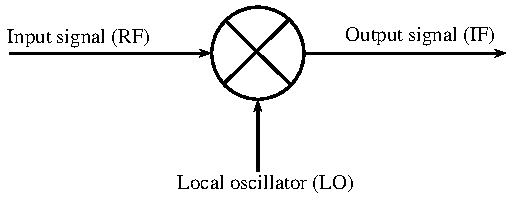
\includegraphics[width=0.6\textwidth]{fig/mixer/mixer.pdf}
				\caption{Schematic component of a mixer.}\label{fig:mixerroughschematic}
			\end{figure}

%			\begin{figure}[hbt!]
%				\centering
%				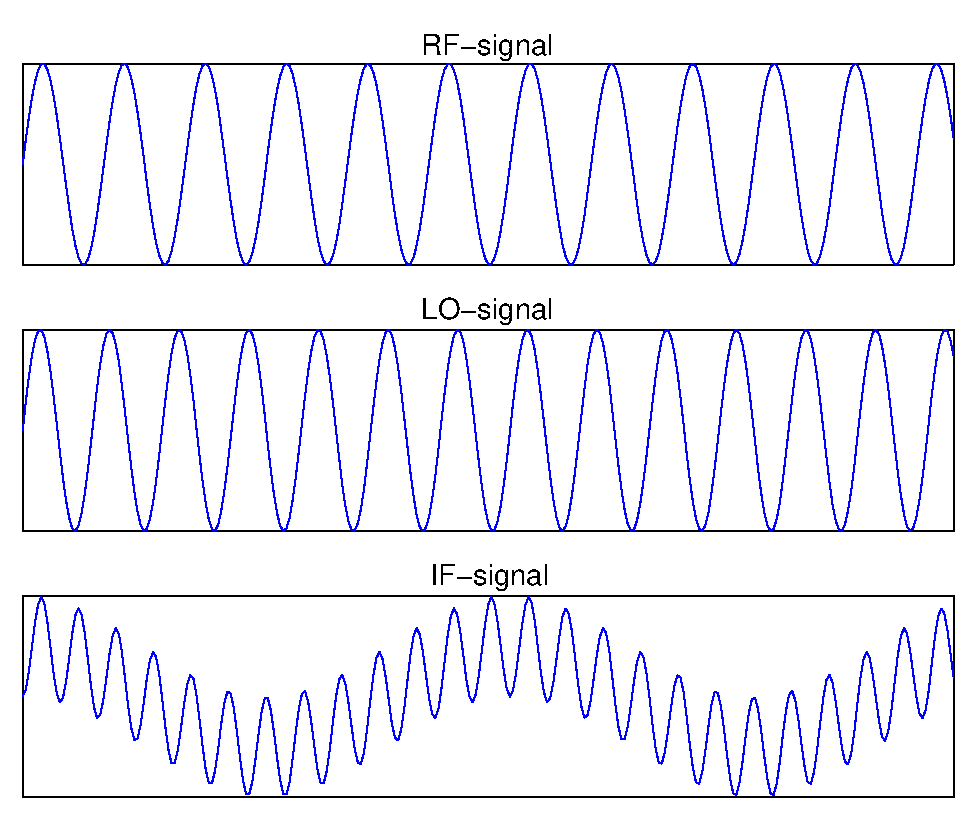
\includegraphics[width=0.6\textwidth]{fig/mixer/mixing_function}
%				\caption{}\label{fig:mixing_function}
%			\end{figure}
			\begin{figure}[hpt!]
				\centering
				\subfloat[][Time domain.]{
					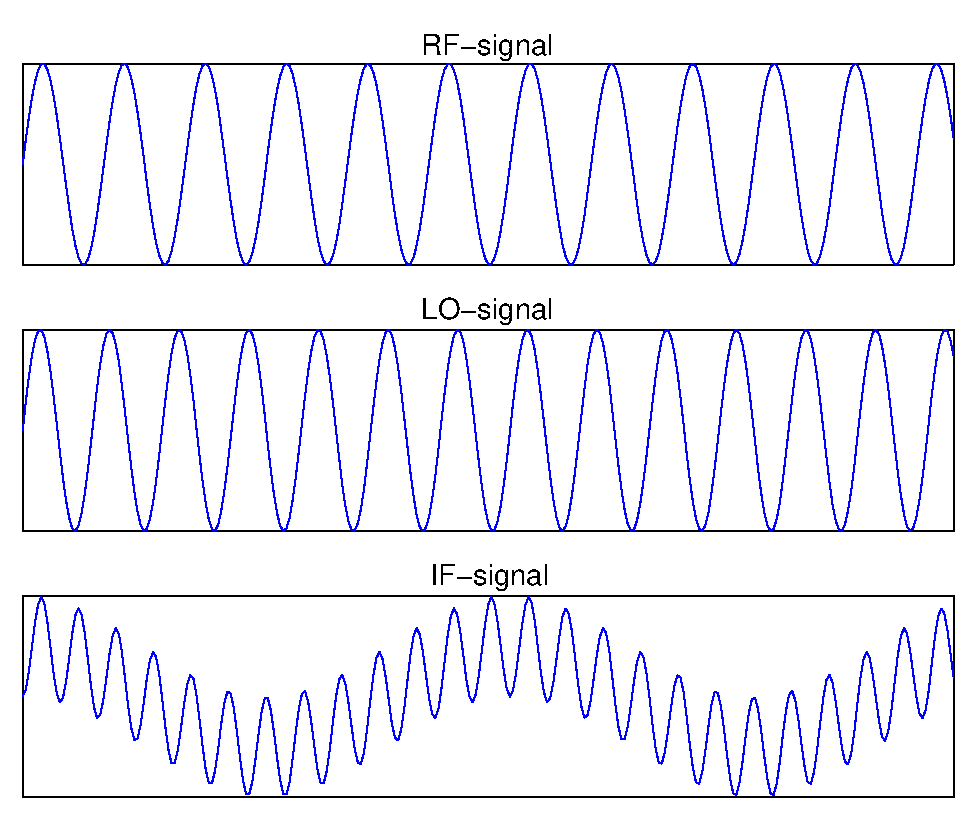
\includegraphics[width=0.5\textwidth]{fig/mixer/mixing_function}
					\label{fig:mixing_function_time}
				}
				\subfloat[][Frequency domain.]{
					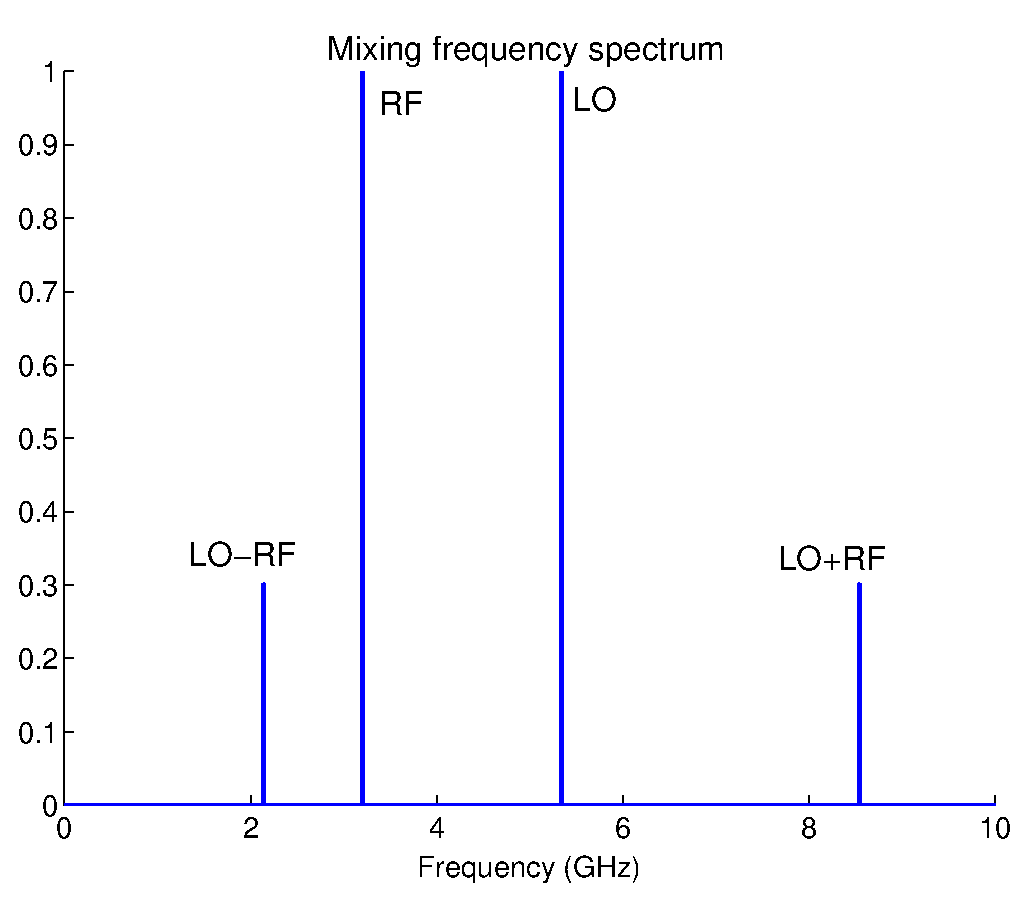
\includegraphics[width=0.5\textwidth]{fig/mixer/mixing_function_fft}
					\label{fig:mixing_function_fft}
				}
				\caption{The resulting signals from multiplication of RF- and LO-signals. The IF-signal contains both the upper and the lower sidebands.}\label{fig:mixing_function}
			\end{figure}

		\subsection{Image rejection}
			An incoming signal in the frequency band that converts to the same IF-frequency as the desired signal is called an image. Once this signal has been down-converted it becomes indistinguishable from the desired signal. To avoid this, the mixer has an image reject specification of \unit[30]{dBc}. This means that the conversion gain of the image should be at least \unit[30]{dB} lower than that of the desired band.


	\section{Intermodulation products}
		\subsection{Linearity and intermodulation}
			The operation of a mixer, or downconverter, should be as linear as possible. Linearity in the mixer ensures as few unwanted signals as possible arise from the mixing procedure. The frequencies of these spurious signals are calculated in the same manner as the downconverted intermediate frequency:\autocite{bahl03}

			\begin{equation}\label{eq:spurs}
				f_{mix} = |k_1f_1\pm k_2f_2 \pm ... \pm k_nf_n|
			\end{equation}

			The order of the intermodulation products are $O=\sum_{m=1}^n|k_m|$ and the amplitude of a signal rapidly decreases as the order gets higher. The intermodulation products that are most harmful are thus low-order signals at frequencies close to the IF. The signal of interest, the IF-signal, will in a non-linear mixer become mixed up with many of these spurious signals. The source of spurious signals are not only different orders of RF and LO signal mixes but also mixes of multiple input RF signals along with the LO. Even though this creates infinite combinations of mixing frequencies, there are a few of special interest. See \citeauthor{kundert02} for a thorough theoretical treatment\autocite{kundert02}.


%			\begin{table}[hbt!]
%			\caption[Two-tone spurious signals.]{Spurious signal frequencies, within \unit[0.5]{GHz} of the IF, originating from a two-tone excitation. The frequencies are mixed according to $f_{mix} = mf_{RF1} + nf_{RF2} + pf_{LO}$ and the orders are $O=|m|+|n|$. $ f_{RF1}=\unit[3.2]{GHz}$, $ f_{RF2}=\unit[3.22]{GHz}$ and $ f_{LO}=\unit[5.34]{GHz}$.}
%			\label{tab:introtwotone}
%			\centering
%			\begin{tabular}{rrrrr}
%				m & n & p & Frequency (GHz) & Order \\\hline
%				  0 &  -6 &   4 & 2.04 & 6 \\
%				  4 &  -5 &   1 & 2.04 & 9 \\
%				 -1 &  -5 &   4 & 2.06 & 6 \\
%				  3 &  -4 &   1 & 2.06 & 7 \\
%				 -2 &  -4 &   4 & 2.08 & 6 \\
%				  2 &  -3 &   1 & 2.08 & 5 \\
%				  6 &  -2 &  -2 & 2.08 & 8 \\
%				 -3 &  -3 &   4 &  2.10 & 6 \\
%				  1 &  -2 &   1 &  2.10 & 3 \\
%				  5 &  -1 &  -2 &  2.10 & 6 \\
%				 -4 &  -2 &   4 & 2.12 & 6 \\
%				  0 &  -1 &   1 & 2.12 & 1 \\
%				  4 &   0 &  -2 & 2.12 & 4 \\
%				 -1 &   0 &   1 & 2.14 & 1 \\
%				 -5 &  -1 &   4 & 2.14 & 6 \\
%				  3 &   1 &  -2 & 2.14 & 4 \\
%				 -6 &   0 &   4 & 2.16 & 6 \\
%				 -2 &   1 &   1 & 2.16 & 3 \\
%				  2 &   2 &  -2 & 2.16 & 4 \\
%				 -3 &   2 &   1 & 2.18 & 5 \\
%				  1 &   3 &  -2 & 2.18 & 4 \\
%				 -4 &   3 &   1 &  2.20 & 7 \\
%				  0 &   4 &  -2 &  2.20 & 4 \\
%				 -5 &   4 &   1 & 2.22 & 9 \\
%				 -1 &   5 &  -2 & 2.22 & 6 \\
%				 -2 &   6 &  -2 & 2.24 & 8
%			\end{tabular}
%			\end{table}

			In order to find out which spurious frequencies are present, all low-order mixing products for the system have been calculated, using frequencies valid for the project (\autoref{tab:introsingletone}). %In the two-tone input two tones of equal amplitude, \unit[20]{MHz} apart, are fed as RF-signals.
			The order of intermodulation by convention only counts the sum of the coefficients of the RF-signals.
		
			\begin{table}[hbt!]
				\caption[Single-tone spurious signals.]{Spurious signal frequencies, within \unit[1.5]{GHz} of the IF, originating from single-tone excitation. The frequencies are mixed according to $f_{mix} = mf_{RF} + nf_{LO}$ and the orders are $O=|m|$. $ f_{RF}=\unit[3.2]{GHz}$ and $ f_{LO}=\unit[5.34]{GHz}$.}
				\label{tab:introsingletone}
				\centering
				\begin{tabular}{rrrr}
					m & n & Frequency (GHz) & Order \\\hline
	%				  4 &  -2 & 2.12 & 4 \\
	%				 -1 &   1 & 2.14 & 1 \\
	%				 -6 &   4 & 2.16 & 6 \\
					  2 &  -1 & 1.06 & 2 \\
					 -3 &   2 & 1.08 & 3 \\
					  4 &  -2 & 2.12 & 4 \\
					 -1 &   1 & 2.14 & 1 \\
					 -6 &   4 & 2.16 & 6 \\
					 -6 &  -3 & 3.18 & 6 \\
					  1 &   0 &  3.2 & 1 \\
					 -4 &   3 & 3.22 & 4
				\end{tabular}
			\end{table}

			A similar calculation of mixing products using two-tone excitation results in more spurious frequencies. The frequencies are mixed according to $f_{mix} = mf_{RF1} + nf_{RF2} + pf_{LO}$, where $f_{RF1}$ and $f_{RF2}$ are placed some tenths of MHz apart. Of special interest are the of $m$ and $n$ low odd-order signals with a low-order LO ($p=1$), and in particular the third-order intermodulation product.

		\subsection{Intercept point} \label{sec:ip3}
			Usually the third-order intermodulation products from multiple input signals cause most distortion. The third-order intercept point is an observable used to quantify the linearity in a component. Although it measures the third-order product in particular, it represents the overall linearity of a system.

			The general $n^{th}$-order intercept point, or $IP_n$, is calculated by exciting the system with two tones, as described above. The intercept point is the theoretical intercept point between the fundamental frequency and the $n^{th}$-order intermodulation product, had the gain (or loss) in the system been linear.\autocite{bahl03,pozar90} That is, for small input (system in linear region) the output of the fundamental signal increases \unit[1]{dB/dB}, and \unit[n]{dB/dB} for the $n^{th}$-order IM product. %Even though the $n^{th}$-order IM product is small for small input it will eventually grow to the same signal strength as the fundamental frequency component.
			The intercept point value is referenced either to the input power ($IIP_n$) or to the output power ($OIP_n$). The two values are determined as illustrated in \autoref{fig:introip3}.

			\begin{figure}[hbt!]
			\centering
			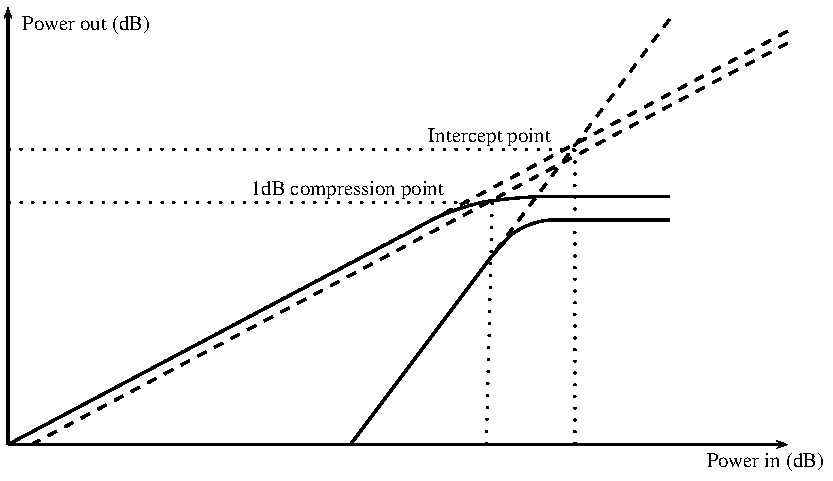
\includegraphics[width=1\textwidth]{fig/introduction/ip3.pdf}
			\caption[Definition of $n^{th}$-order intercept point and 1 dB compression point.]{The theoretical intercept point between the fundamental frequency component and an intermodulation product. The \unit[1]{dB} compression point ($P_{1dB}$) is marked as well.}\label{fig:introip3}
			\end{figure}

		\subsection{\unit[1]{dB} compression point}\label{sec:p1db}
			The \unit[1]{dB} compression point ($P_{1dB}$) is another measure of linearity. It is the point at which the output power is compressed \unit[1]{dB} compared to the linear case (\autoref{fig:introip3}). This measure is also referenced to either the input or the output power.

			$P_{1dB}$ is shown to be approximately \unit[10]{dB} lower than $IIP_3$.\autocite{kundert02} It can therefore be used as a second parameter to estimate and verify the linearity of a component in the design phase. %For the mixer component it's essential, as the simulation software is unable to apply the necessary simulation accuracy for a three-tone setup needed to calculate $IP_3$.

		\subsection{Cascaded components}\label{sec:casc_iip3}
			As circuits usually contain multiple components, such as amplifiers, mixers, filters etc, it is preferable to treat the linearity of each component individually in the design process. The total $IIP_3$ for two components is then given by \autocite{pozar90}

			\begin{equation}\label{eq:casciip3}
				I_T=\left ( \frac{1}{G_2I_1} + \frac{1}{I_2} \right )^{-1}
			\end{equation}

			$I_1$, $I_2$ and $I_T$ are the $IIP_3$ for the first component, second component and the two together, respectively. $G_2$ is the gain of the second device in the cascade. It is here evident that the order of the components are important for the total linearity.

		\subsection{Linearity simulations}
			In order to simulate a mixer's $IIP_3$ a three-tone setup is required (LO and two input RF tones). Necessary simulation accuracy for all three tones and their mixing products is very high, too high for the simulation software Microwave Office to handle. In contrast to the simpler two-tone setup required for calculating $IIP_3$ in an amplifier, the result becomes unreliable.

			The theory that results in the rule of thumb $IIP_3=P_{1dB}+\unit[10]{dBm}$ is based on a power series expansion of the transfer characteristics. A simplification to the calculations is made to only consider the first three terms. This approximation has been empirically shown to work well with amplifiers. In mixers, there are however much more harmonics present and they cannot be as easily discarded. A quick look at different papers and commercial mixers show that $IIP_3$ can be anything from \unit[6]{dBm} to \unit[14]{dBm} higher than $P_{1dB}$.

			This means that neither an estimate of $IIP_3$ from $P_{1dB}$ nor a simulation of $IIP_3$ directly are reliable methods for the mixer. The two combined gives the best hint available to a correct $IIP_3$ value.

	\section{Noise}
		\subsection{Noise sources}\label{sec:noise_thermal}
			Thermal noise arise due to collisions between electrons. As temperature increases, the particles will move faster and collide more often, thus increasing the thermal noise. The mean-square thermal noise voltage generated in a resistance $R$ over a bandwidth $\Delta f$ is\autocite{bahl03}

			\begin{equation}
				< v^2_\text{thermal} > = 4k_BTR\Delta f
			\end{equation}

			This type of noise is introduced in passive, resistive components such as resistors and inductors.

			A second type of noise present in active structures such as the FETs is shot noise. Shot noise occurs when there are not enough electrons to successfully approximate the current as continuous. The statistical variations in the electron's speed result in the sum of all electrons having variations as well. The mean-square shot noise voltage for a current $i$ which flows through resistance $R$ is given by
			\begin{equation}
				< v^2_\text{shot} > = 2q_eiR^2\Delta f
			\end{equation}

		\subsection{Noise in a system}
			When designing electrical circuits in general and receivers in particular, the noise must be considered at every step. Without proper design, it will be problematic to differentiate signals from the background noise. Noise has all kinds of origins; it is part of the original transmission and it is introduced while processing the signal.

			An important measure when dealing with noise is the signal to noise ratio, or SNR, which is the ratio between the useful signal and the underlying noise. It is defined as
			\begin{equation}
					\text{SNR}=20\log \left(\frac{ A_\text{signal} }{ A_\text{noise} }\right)
			\end{equation}
			where $A$ is the amplitude of the signal. In \autoref{fig:noise_example}, examples with different SNR are shown.

			\begin{figure}[hb!!!]
				\centering
				\subfloat[][]{
					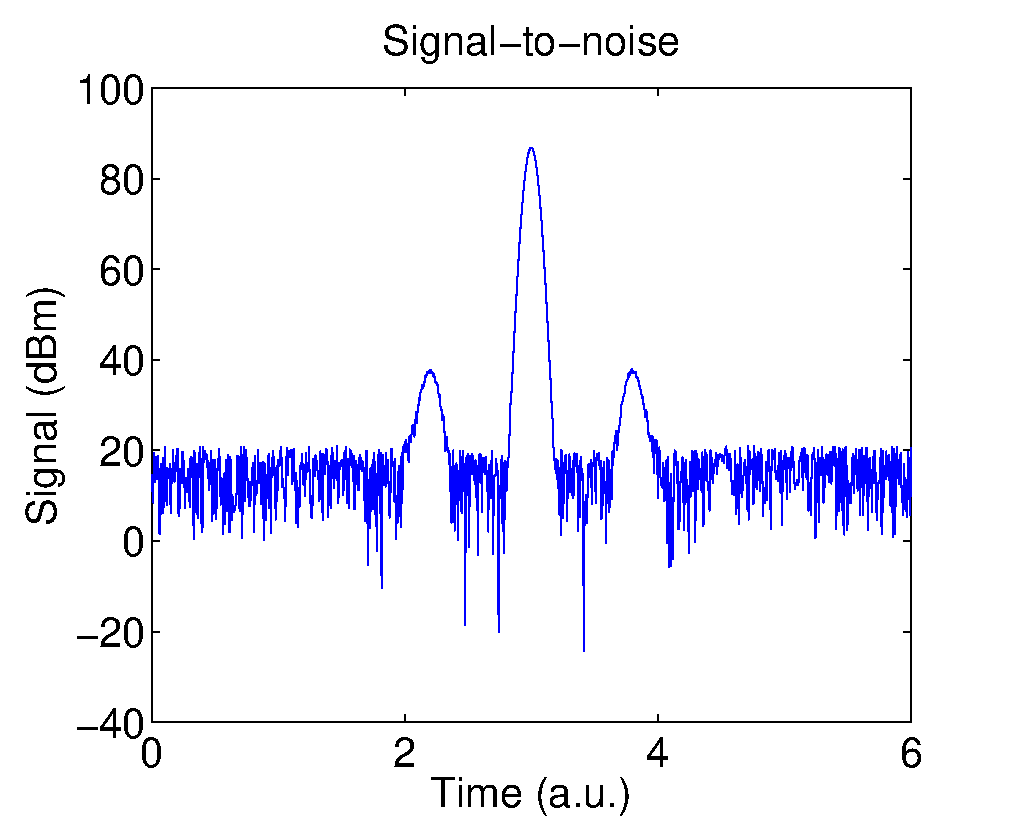
\includegraphics[width=0.5\textwidth]{fig/introduction/noise_example.eps}
					\label{fig:intro_noise_example}
				}
				\subfloat[][]{
					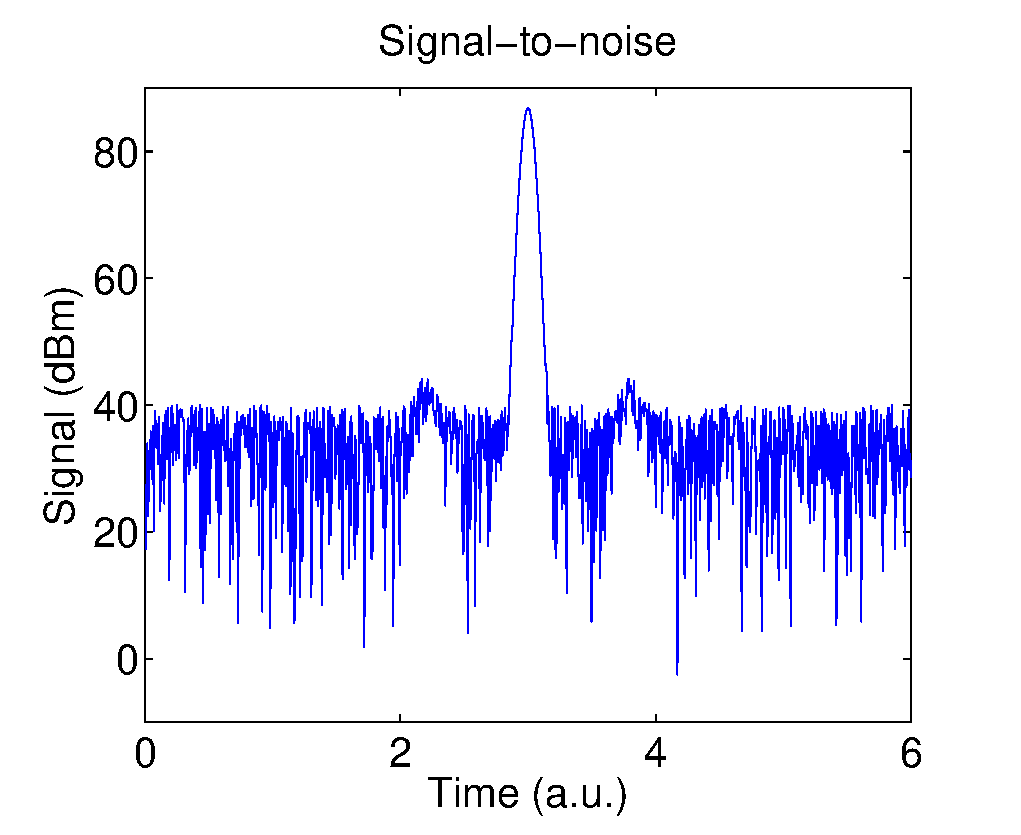
\includegraphics[width=0.5\textwidth]{fig/introduction/noise_example_2.eps}
					\label{fig:intro_noise_example_2}
				}
				\caption[Example of signal plus noise.]{\subref{fig:intro_noise_example} An example of how noise makes it difficult to measure anything but the very strong signals. The noise level and the strongest signal are found at \unit[20]{dBm} and \unit[87]{dBm}, respectively. This results in a SNR of \unit[67]{dBm}. In \subref{fig:intro_noise_example_2} the environment is noisier. The side lobes are barely visible.}\label{fig:noise_example}
			\end{figure}

		\subsection{Noise figure}
			The noise figure, or $\nf$, measures how much noise a subcircuit introduces. Introducing noise is inevitable and in order to minimize the noise, it is important to amplify the signal as early as possible and thereby raising the signal higher above the background noise. Otherwise, every subsequent attenuation of the signal will raise the noise figure just as much. $\nf$ is defined as

			\begin{equation}
				\nf=10\log \left(\frac{ \text{SNR}_\text{in} }{ \text{SNR}_\text{out} }\right) = \text{SNR}_\text{in,dB} -\text{SNR}_\text{out,dB}
			\end{equation}

			For example, in Figure\autoref{fig:intro_noise_example}, the SNR is \unit[67]{dB}. If the same ratio were to be \unit[47]{dB} after some passing through some component as in Figure\autoref{fig:intro_noise_example_2}, the noise figure for this component would be \unit[20]{dB}.


		\subsection{Cascaded components}
			The total noise figure (\nf) for a system with two components is given by \autocite{pozar90}

			\begin{equation}
				\nf_T=\nf_1+\frac{1}{G_1}(\nf_2-1)
			\end{equation}

			where $\nf_1$, $\nf_2$ and $\nf_T$ are the noise figures of the first component, the second component and the total system respectively. $G_1$ is the gain of the first component. Just as for $IIP_3$ the order of the components plays a big part of the final noise figure. In the next chapter different permutations of components are analysed for the purpose of finding which components and what order give the best trade-off between noise and linearity.
